\section{Reševanje}
\subsection{Podnaloga 1}
Najprej se uverim, da lahko iz začetnih pogojev pravilno integriram časovni
razvoj. Izbral sem si nekaj začetnih hitrosti, za katere vemo, kakšne orbite
porodijo. Za orbite\footnote{brez upoštevanja simetrije $v_0 \rightarrow - v_0$
    in izrojenih elips za $v_0 = 0$} velja:
\[
    \mathrm{orbita}=\begin{cases}
        \mathrm{kro\check{z}nica}, & v_0 = 1,        \\
        \mathrm{hiperbola},        & v_0 = \sqrt{2}, \\
        \mathrm{parabola},         & v_0 > \sqrt{2}, \\
        \mathrm{elipsa},           & \mathrm{sicer}
    \end{cases}
\]
\begin{samepage}
    Za \(v_0 \in \{ 1, \sqrt{2}, 1.5, 0.7 \}\) sem izračunal trajektorije v
    časovnem intervalu $ t\in\left[ 0, 10\right] $ z adaptivnim časovnim korakom
    z metodo \texttt{scipy.integrate.solve\_ivp}. Na spodnji sliki vidimo, da
    dobimo pričakovane trajektorije:

    \begin{center}
        \centering
        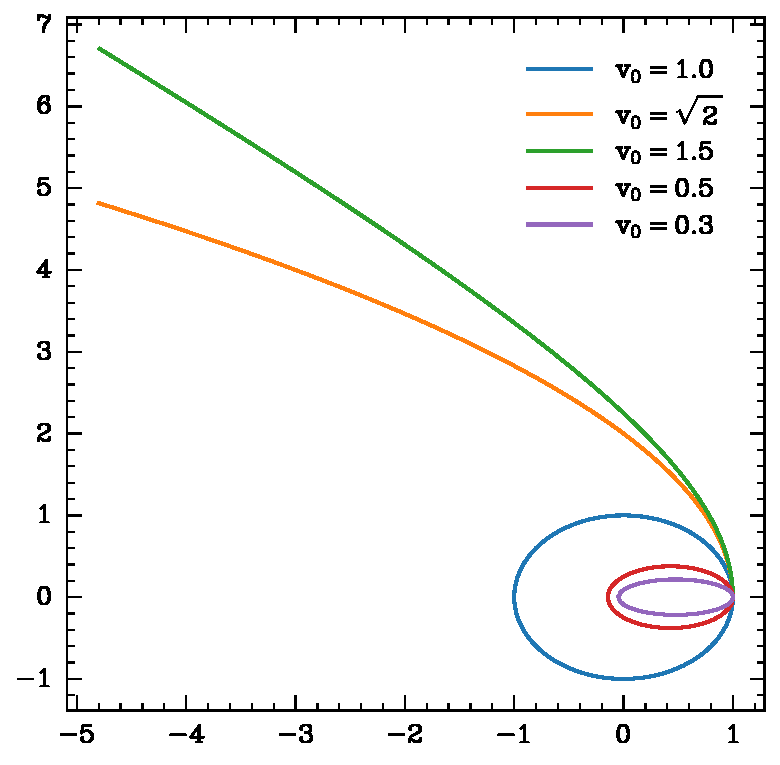
\includegraphics[width=0.8\textwidth]{../images/1-1-v0.pdf}
    \end{center}
\end{samepage}

Naslednji korak je študija invariantnih količin. Zanimalo nas bo spreminjanje
polne energije $H$, vrtilne količine $\mathbf{L}$,  in Laplace-Runge-Lenzovega
vektorja $\mathbf{A}$ skozi čas za različne začetne pogoje. Rezultate prikazujem
na sliki~\ref{fig:1-1_invariantne_kolicine}.

\begin{figure}
    \centering
    \begin{subfigure}{0.48\textwidth}
        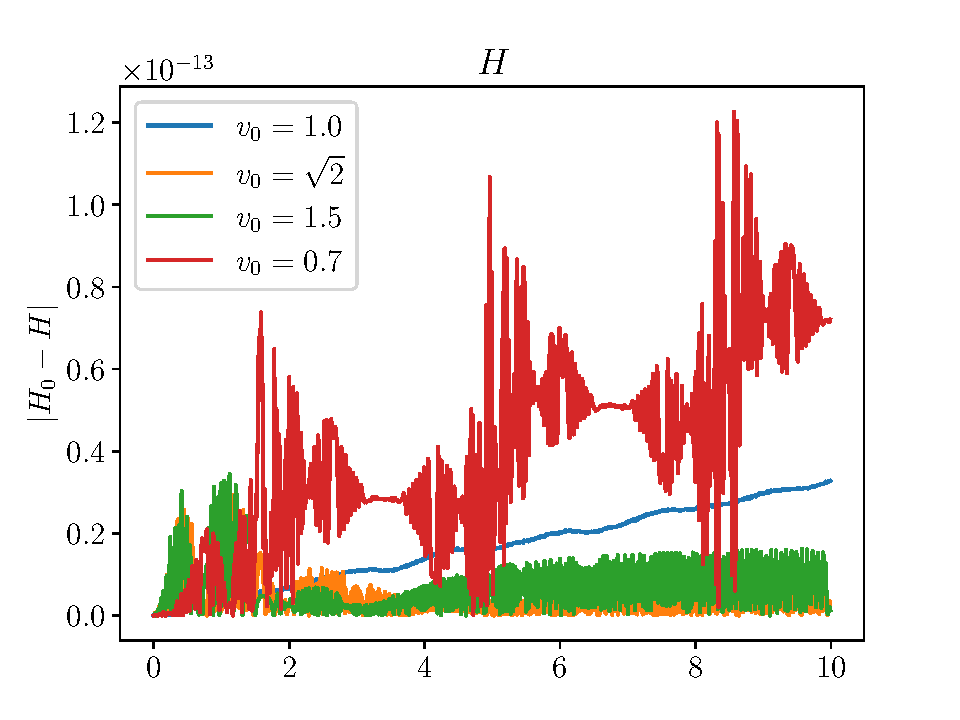
\includegraphics[width=\textwidth]{../images/1-1-H_lin.pdf}
    \end{subfigure}
    \hfill
    \begin{subfigure}{0.48\textwidth}
        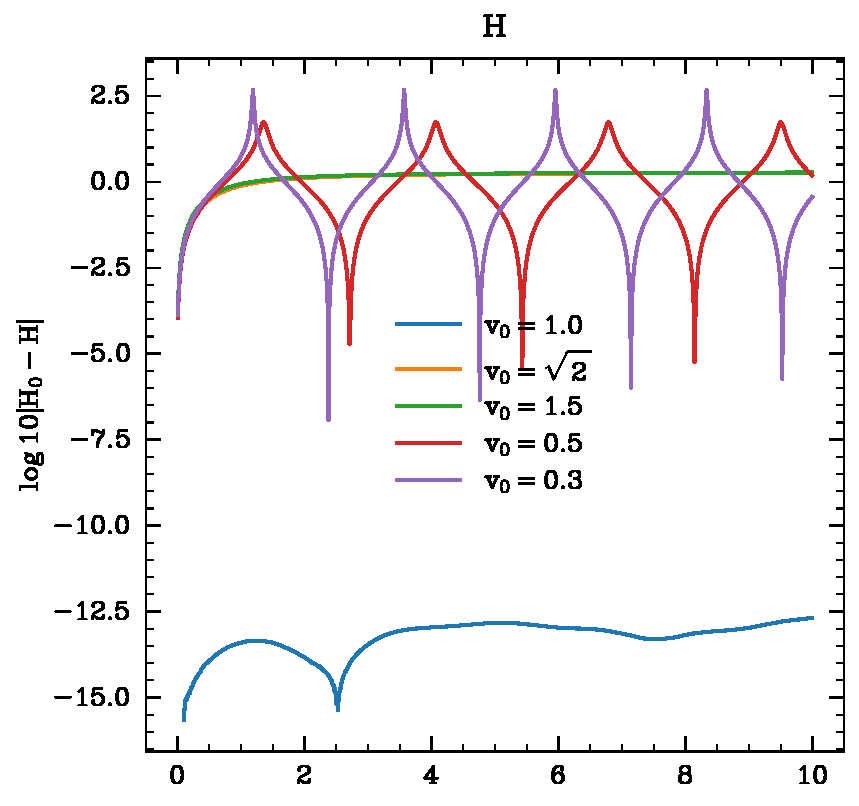
\includegraphics[width=\textwidth]{../images/1-1-H_log.pdf}
    \end{subfigure}
    \newline
    \begin{subfigure}{0.48\textwidth}
        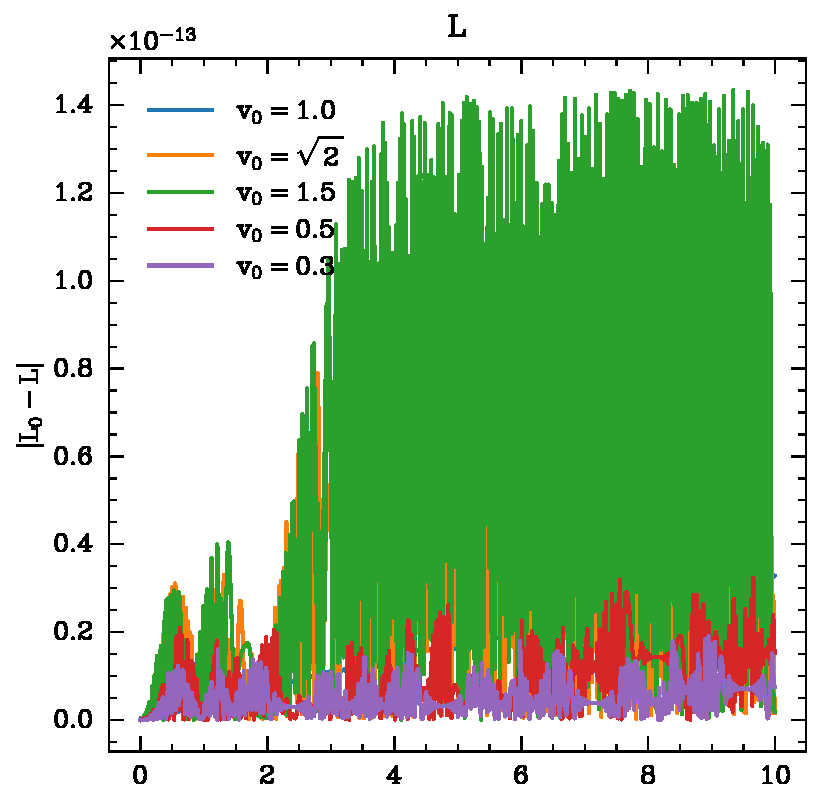
\includegraphics[width=\textwidth]{../images/1-1-L_lin.pdf}
    \end{subfigure}
    \hfill
    \begin{subfigure}{0.48\textwidth}
        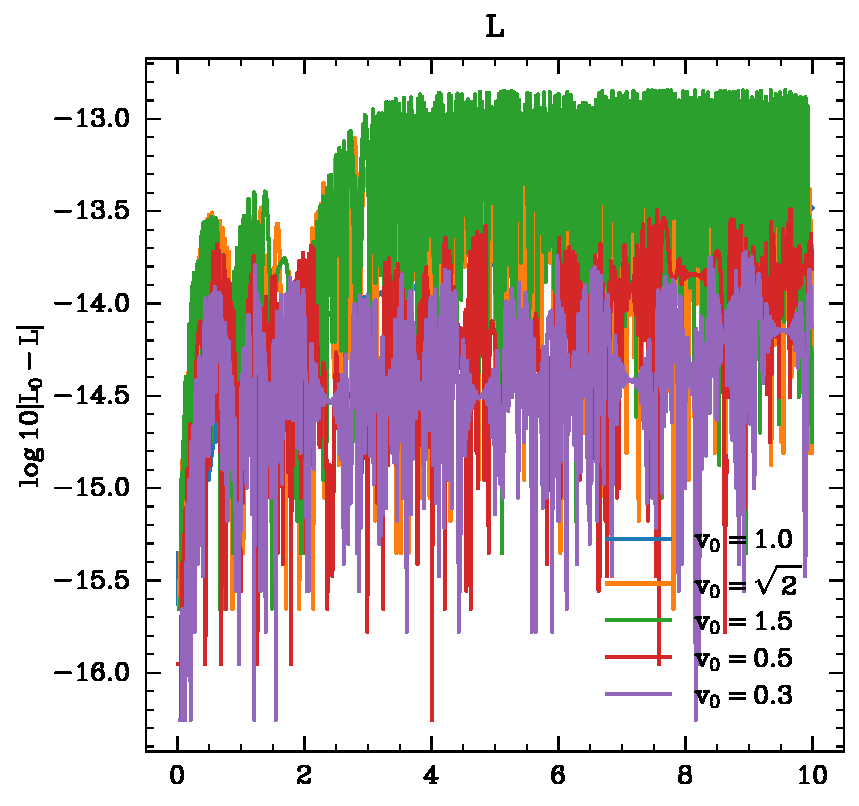
\includegraphics[width=\textwidth]{../images/1-1-L_log.pdf}
    \end{subfigure}
    \newline

    \begin{subfigure}{0.48\textwidth}
        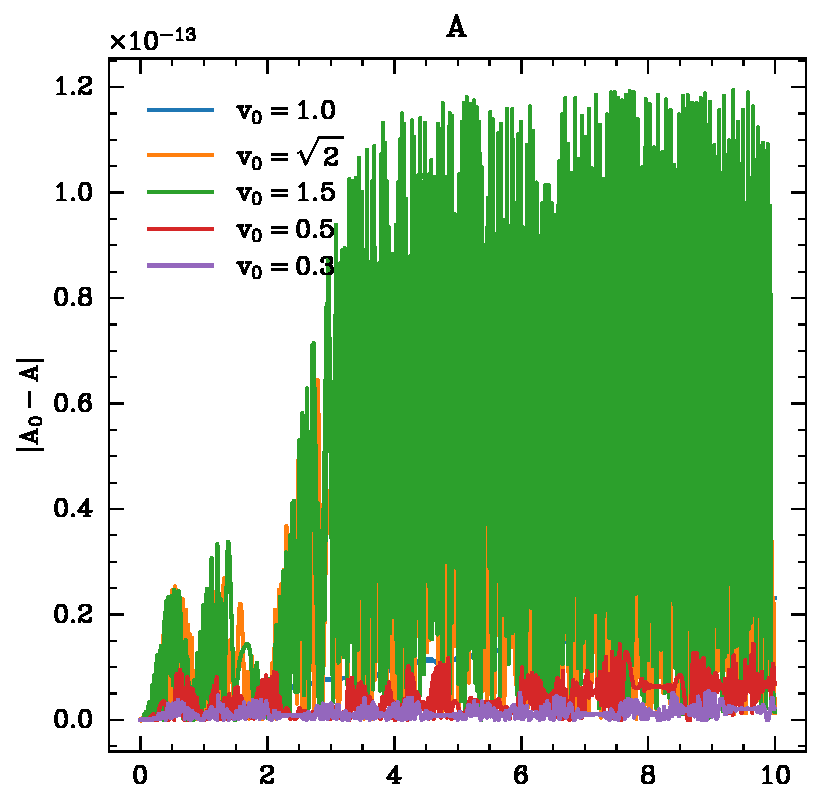
\includegraphics[width=\textwidth]{../images/1-1-A_lin.pdf}
    \end{subfigure}
    \hfill
    \begin{subfigure}{0.48\textwidth}
        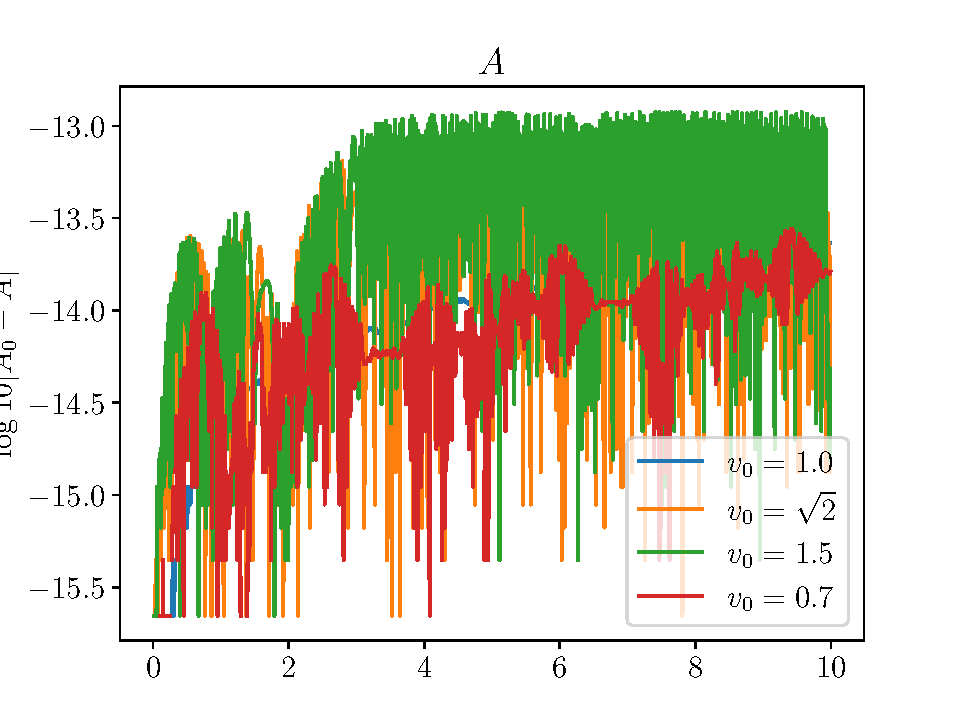
\includegraphics[width=\textwidth]{../images/1-1-A_log.pdf}
    \end{subfigure}

    \caption{ Časovni poteki invariantnih količin. Opazimo, da za izbrano
        integracijsko shemo niso stabilne, marveč se skozi integracijo
        spreminjajo.    Obnašanje količin za različne pogoje so korelirane; pri
        $v_0=1$ vedno opazimo umirjen `drift' količine, za druge začetne pogoje
        pa je dinamika lahko bolj divja; opazimo območja konstantnosti in
        območja divjih fluktuacij.}
    \label{fig:1-1_invariantne_kolicine}
\end{figure}

\clearpage

Za študijo stabilnosti obhodnih časov sem implementiral t.i.~\emph{event tracker},
funkcijo, katere koren bo integrator iskal:

\begin{minted}[linenos]{python}
initial = [1, 0, 0, v0]
def complete_revolution(t, y):
    return y[1]
complete_revolution.terminal = False
complete_revolution.direction = 1

sol = solve_ivp(odes,
    t_span=[0, 50*np.pi],
    y0=initial,
    dense_output=True,
    events=complete_revolution,
)
\end{minted}

Pri tem sem se posvetil primerom, ko $v_0<\sqrt{2}$, da zagotovim periodičnost
orbit. Uporabljena je bila sledeča metodologija: za vsak $v_0$ sem iskal orbito
za $t\in \left(0, 50\pi \right)$, pri čemer mi je prehode čez $y=0$ iskal
integrator sam.  Dobljene čase prehoda sem numerično odvajal, da dobim čase med
zaporednimi prehodi, nato pa sem izračunal povprečno periodo in standardno
deviacijo. Rezultate prikazujem na naslednji sliki.


\begin{center}
    \centering
    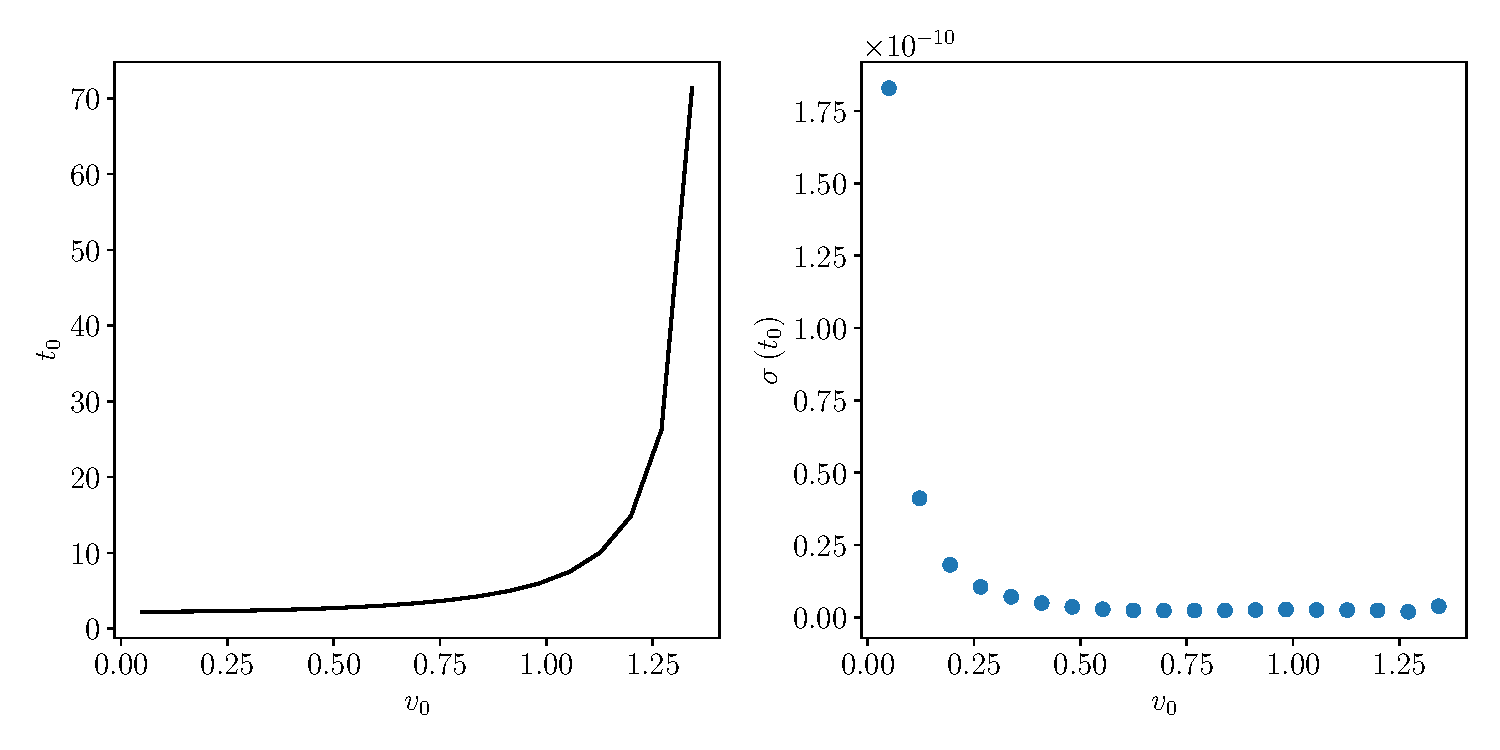
\includegraphics[width=0.9\textwidth]{../images/1-2-t0_abs.pdf}
    {Stabilnost obhodnega časa $t_0$ kot funkcija začetne hitrosti planeta~$v_0$. [\textsc{Levo}] povprečne vrednosti zaporednih
        obhodnih časov s standardnimi deviacijami. [\textsc{Desno}] standardne
        deviacije intervalov med zaporednimi prehodi.}
    % \label{fig:1-2-t0}
\end{center}

Pri nizkih začetnih hitrostih standardna deviacija zaporednih izmerkov strmo
naraste, vzrok česar bi lahko bila težja integracija v bližini pola potenciala.

Ker je pri vseh integracijah doslej za časovni korak skrbel integrator sam, si
pogledam še odvisnost rezultatov od izbire časovnega koraka, ki bo to pot podan
eksplicitno, za integrator pa namesto \texttt{scipy.integrate.solve\_ivp}
uporabim  metodo \texttt{scipy.integrate.ode}. Kot prej bom integriral krožno
trajektorijo in zanjo izračunal invariantne količine skozi čas integracije. Ker
vemo, da bi morale biti konstantne, lahko za merilo kvalitete integracije
izberemo številne metrike. V mojem primeru sem izbral standardno deviacijo in
generiral spodnjo sliko:

\begin{center}
    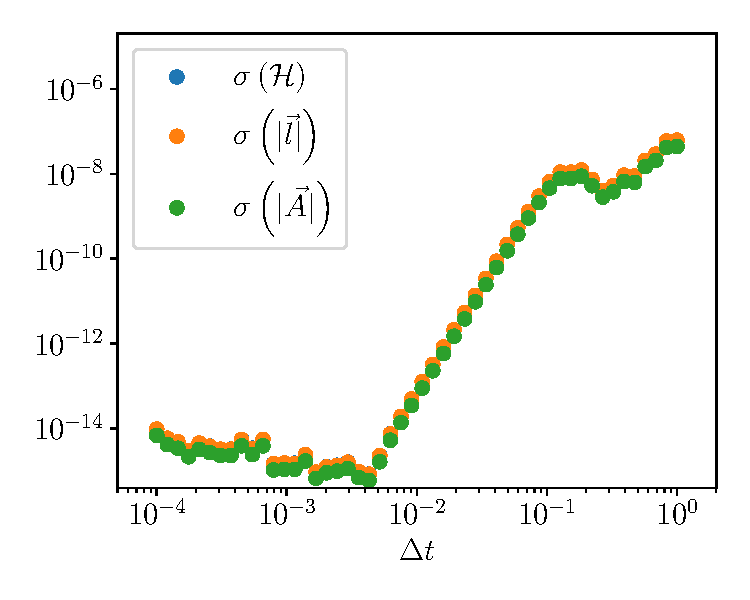
\includegraphics[width=0.5\textwidth]{../images/1-stds.pdf }
\end{center}

Sprva nisem pričakoval, da bo dobljen profil nemonotona funkcija časovnega
koraka $\Delta t$. Visoka razpršenost izmerkov pri velikih $\Delta t$ je trivialna,
ponovno naraščanje v režimu $\Delta t < \Delta t_{\text{optimal}}$ pa bi lahko
pripisali akumulaciji napak zaradi visokega števila korakov.
\clearpage

\subsection{Podnaloga 2}

Cevovod za integracijo sem popravil tako, da je upošteval prispevek dveh
polsonc, ki krožita okrog skupnega težišča z nastavljivo kotno hitrostjo,
nastavljivo medsebojno razdaljo, in nastavljivim zamikom glede na planet.

Raziskal sem, kakšne orbite lahko dobim z različnimi nastavitvami začetnih
parametrov. Z rumeno prikazujem orbiti sonc.
\begin{center}
    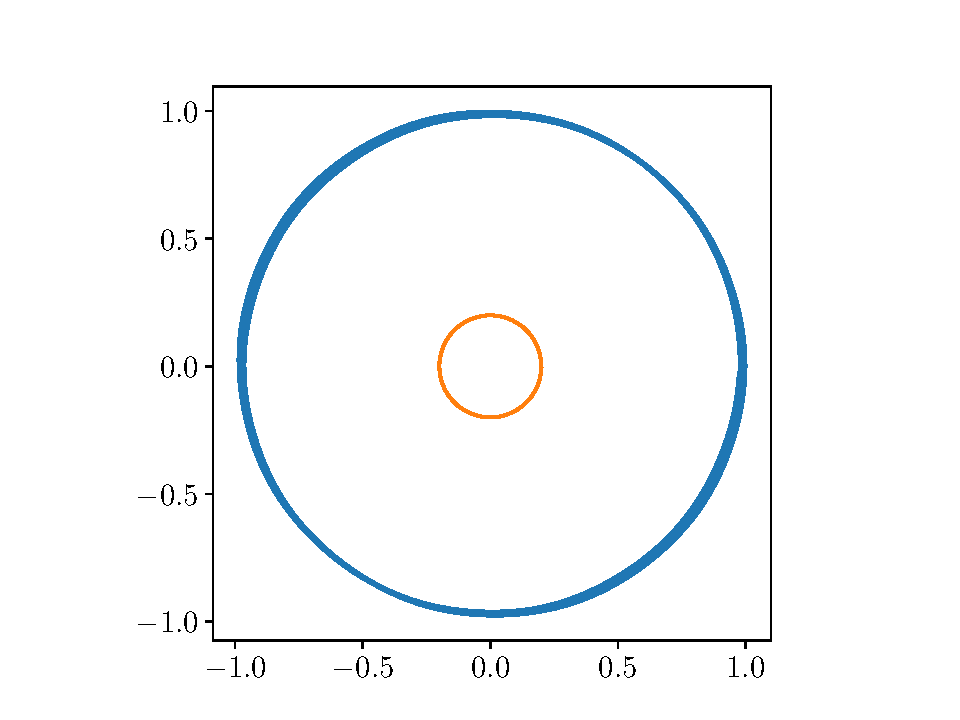
\includegraphics[width=0.5\textwidth]{../images/2-1-orbite_1.pdf}\hfill
    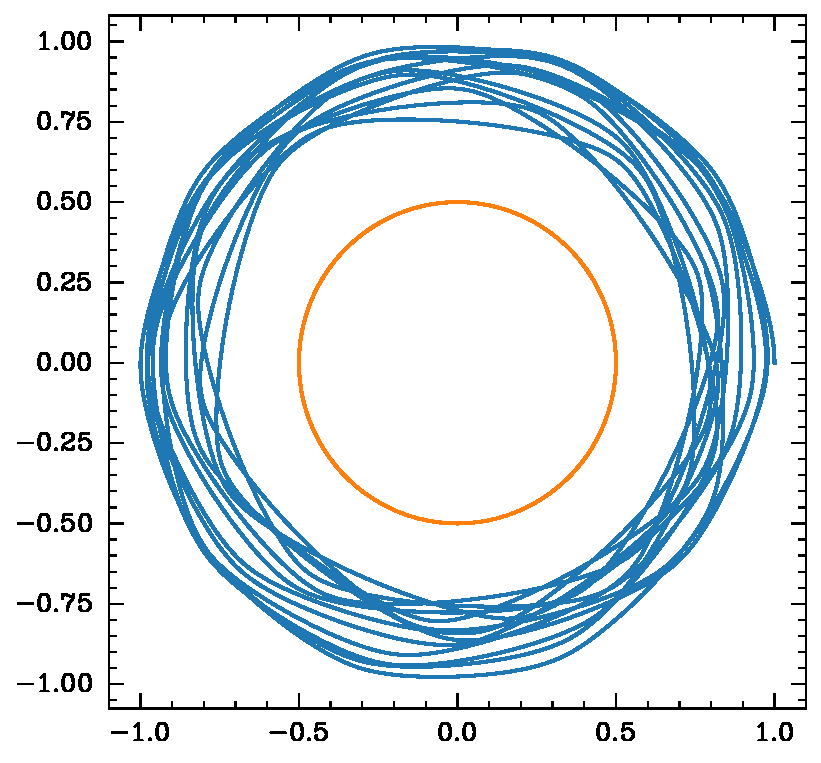
\includegraphics[width=0.5\textwidth]{../images/2-1-orbite_2.pdf}

    % \includegraphics[width=0.5\textwidth]{../images/2-1-orbite_3.pdf}\hfill
    % \includegraphics[width=0.5\textwidth]{../images/2-1-orbite_4.pdf}
\end{center}

Za študijo vpliva dvozvezdja na dinamiko planeta pogledam krožne orbite planeta
pri $v_0 = 1$. Z variacijo razdalje med polsoncema~$r$ opazujem, kaj se dogaja s
povprečjem in standardno deviacijo oddaljenosti  orbite planeta od masnega
središča sistema. V analizo sem vključil samo primere, kjer planet ne 'pobegne'.
Kotna hitrost polsonc je v vseh poskusih znašala $2\pi$. Trajektorije sem
integriral do časa $t=60$, začetna hitrost planeta je bila fiksirana na $v_0=1$.

Kot pričakovano je vpliv večji pri večjih medzvezdnih razdaljah, ko $r
    \rightarrow d$, viden pa je že pri majhnih. Presenetljivo je vpliv
dvozvezdja bolj opazen, ko je ob času~0 zveznica med polsoncema navpična.

\begin{center}
    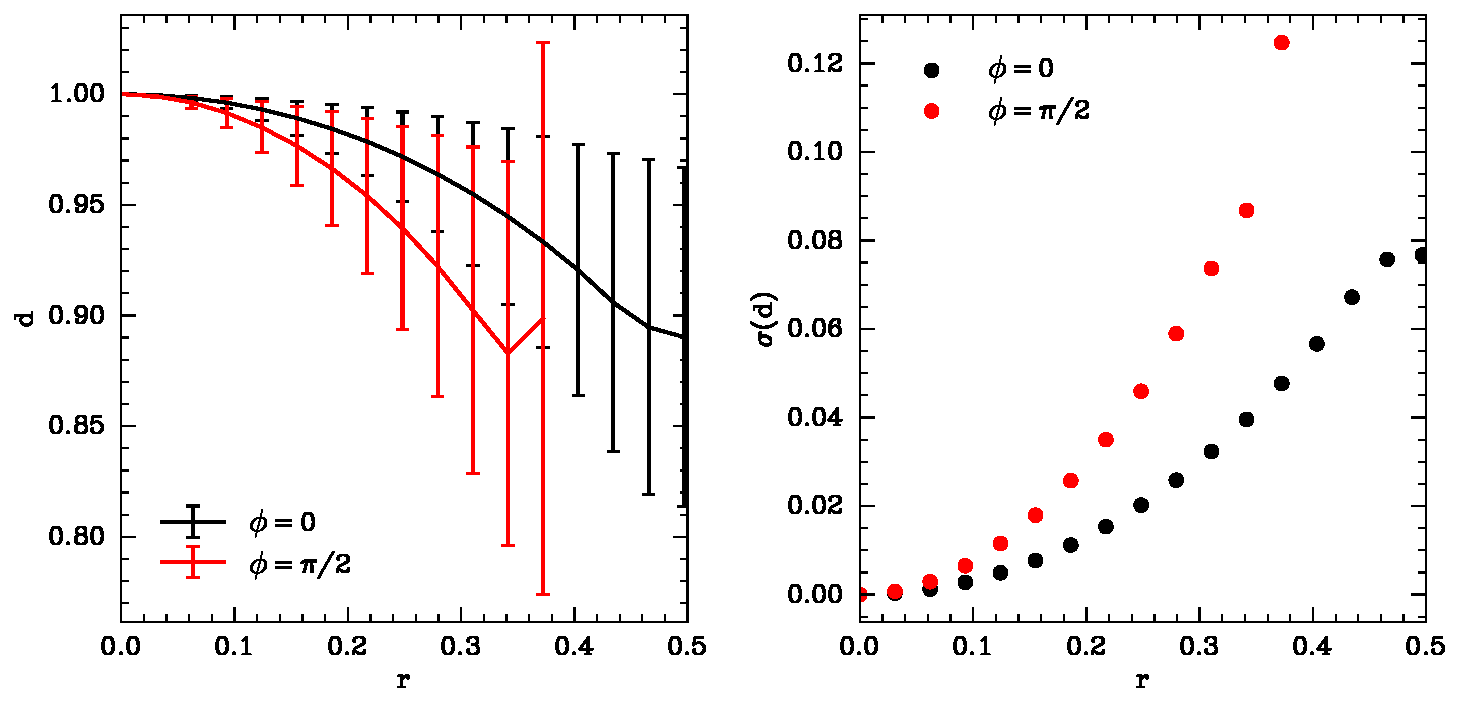
\includegraphics[width=0.9\textwidth]{../images/2-2-vplivr.pdf}
\end{center}

Če definiramo vezanost planeta preko polne energije
\[
    H = T - \frac{0.5}{d_1} - \frac{0.5}{d_2} = \begin{cases}
        > 0    & \implies \text{nevezan}; \\
        \leq 0 & \implies \text{vezan}
    \end{cases},
\]

lahko za fiksen čas integracije in fiksne začetne pogoje pogledamo odvisnost
`usode' planeta v ravnini $(\omega, \phi)$. Pri pregledu ravnine sem kot poprej
fiksiral začetne pogoje  na  $y_0 = \left[ 1,0,0,1\right]$,  medsebojno razdaljo
polsonc pa nastavil na $r=0.5$. V koordinati~$\phi$ pričakujemo simetrijo, saj
je konfiguracija s $\phi = 2\pi$ enaka kot $\phi=0$, poleg tega pa sta polsonci
enaki, zato dobimo pri $\phi=\pi$ enake pogoje kot pri~$\phi=0$. V
koordinati~$\omega$ take simetrije nimamo, in po predhodno prikazanih trajektorijah
gre sklepati, da lahko pričakujemo bogato in netrivialno dinamiko.

\begin{center}
    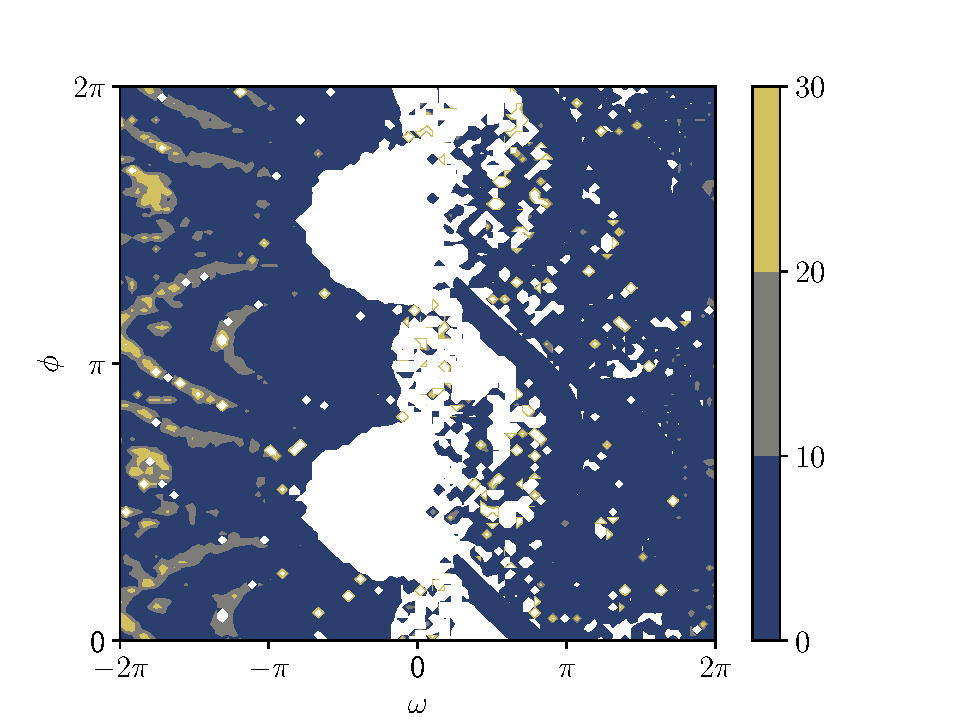
\includegraphics[width=0.5\textwidth]{../images/2-3-fazni-prostor-.pdf}\hfill
    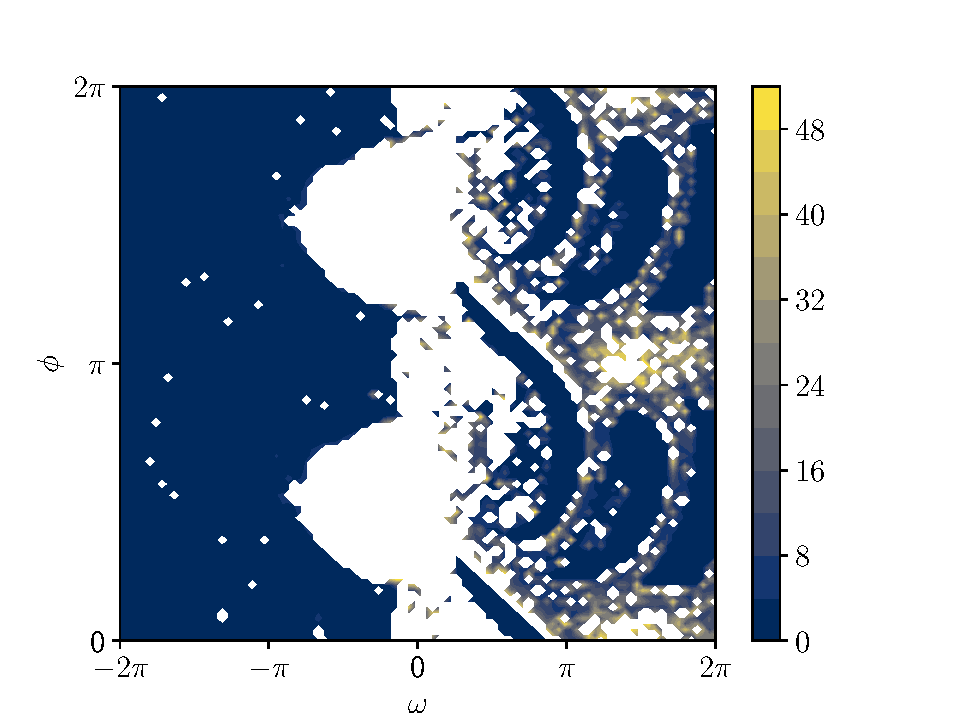
\includegraphics[width=0.5\textwidth]{../images/2-3-escape_time.pdf}
    {Obravnava `usode' planeta. [\textsc{Levo}] Polna energija planeta po času $t=50$.
        Bela barva označuje vezano stanje z nepozitivno polno energijo, ostale barve
        pa nevezano stanje s pozitivno polno energijo. [\textsc{Desno}] Čas, pri
        katerem  dosežemo nevezano stanje.

    }
\end{center}




\subsection{Podnaloga 3}

Za študijo preleta mimobežne zvezde sem spet pripravil cevovod za integracijo.
Tokrat sem poleg koordinat in impulzov planeta integriral še vodoravno
koordinato mimobežne zvezde, kar sem lahko uporabil kot signal za končanje
terminacije (kot opisano v prvi podnalogi.) Za začetne pogoje vzamem
\[
    y_0 =
    \begin{bmatrix}
        x \\
        y \\
        v \\
        u \\
        x_2
    \end{bmatrix} =
    \begin{bmatrix}
        \cos{\phi}        \\
        \sin{\phi}        \\
        - v_0  \sin{\phi} \\
        v_0    \cos{\phi} \\
        -10
    \end{bmatrix},
\]

kjer je $x_2$ vodoravna koordinata mimobežne zvezde. Parametra $\phi$ in $v_0$
si pustim prosta za eksperimentacijo. Za boljši uvid integracijo pustim teči
dlje kot naloga zahteva, nato pa po izračunanih trajektorijah izračunam energije
$H$, $H_1$, in $H_2$, definirane kot:
\begin{align*}
    T_1 & = \frac{u^2 +v^2}{2}               \\
    T_2 & = \frac{(u-u_2)^2 + (v-v_2)^2}{2}  \\
    d_1 & = \sqrt{(x - 0)^2 + (y - 0)^2}     \\
    d_2 & = \sqrt{(x - x_2)^2 + (y - 1.5)^2} \\
    % H   & = T - \frac{0.5}{d_1} - \frac{0.5}{d_2} \\
    H_1 & = T_1 - \frac{0.5}{d_1}            \\
    H_2 & = T_2 - \frac{0.5}{d_2},
\end{align*}


S preletom parametrskega prostora lahko najdem nekaj zanimivih primerov, kjer
mimoleteče sonce spremeni orbito planeta, s svojim gravitacijskim privlakom
izbije planet iz prvotne orbite, ali pa potegne planet za seboj. Najdem lahko tudi nekaj primerov, kjer
planet trči v mimobežno sonce, kar v praksi izgleda kot odpoved integratorja zaradi numerične nestabilnosti

\begin{center}
    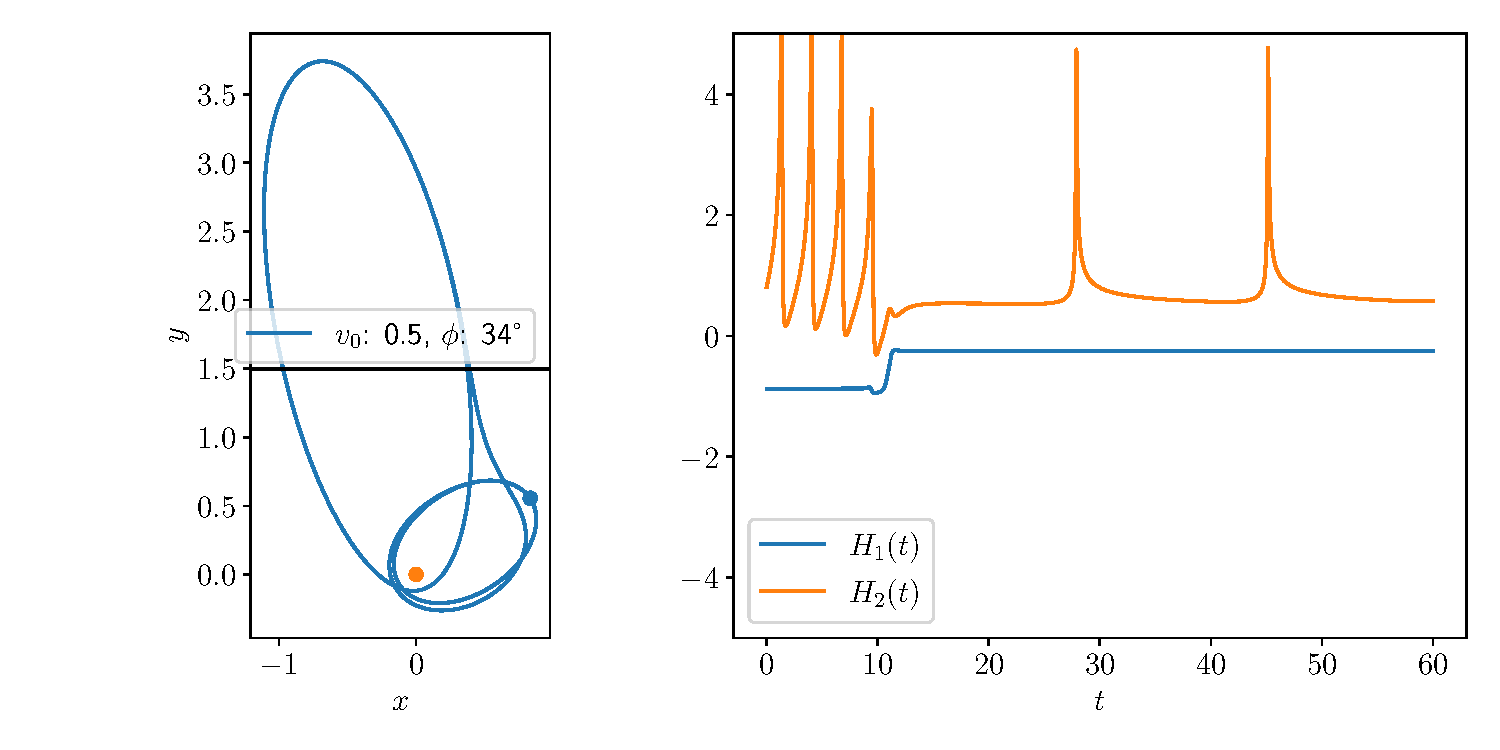
\includegraphics[width=0.9\textwidth]{../images/3-1-3.pdf}\\
    Zaradi privlaka zvezde mimobežnice se spremeni polna energija in vrtilna količina planeta,
    vendar še vedno ostane vezan na prvotno zvezdo.
\end{center}
\begin{center}
    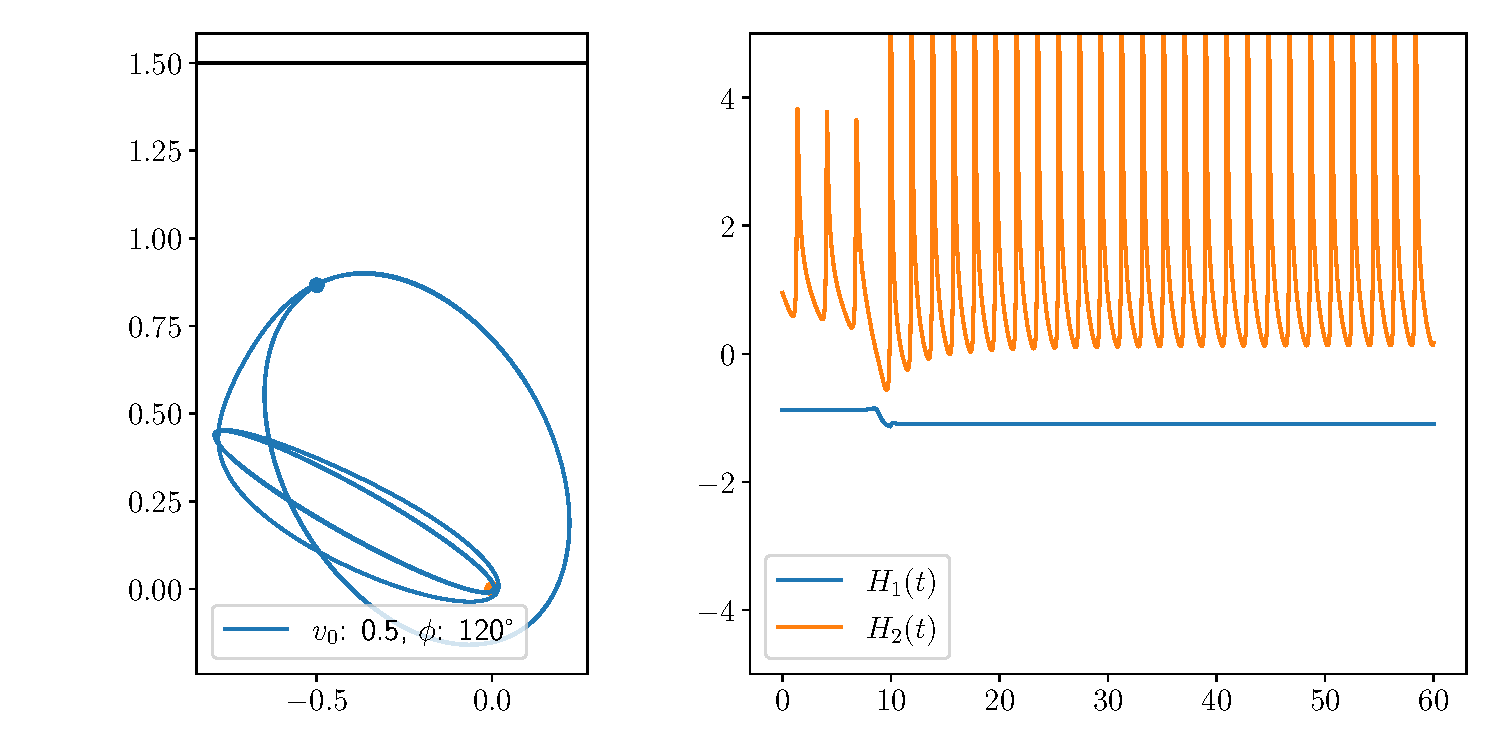
\includegraphics[width=0.9\textwidth]{../images/3-1-6_.pdf}\\
    Sličen primer, vendar v tem primeru mimobežnica 'zavre' planet.
\end{center}

\begin{center}
    % 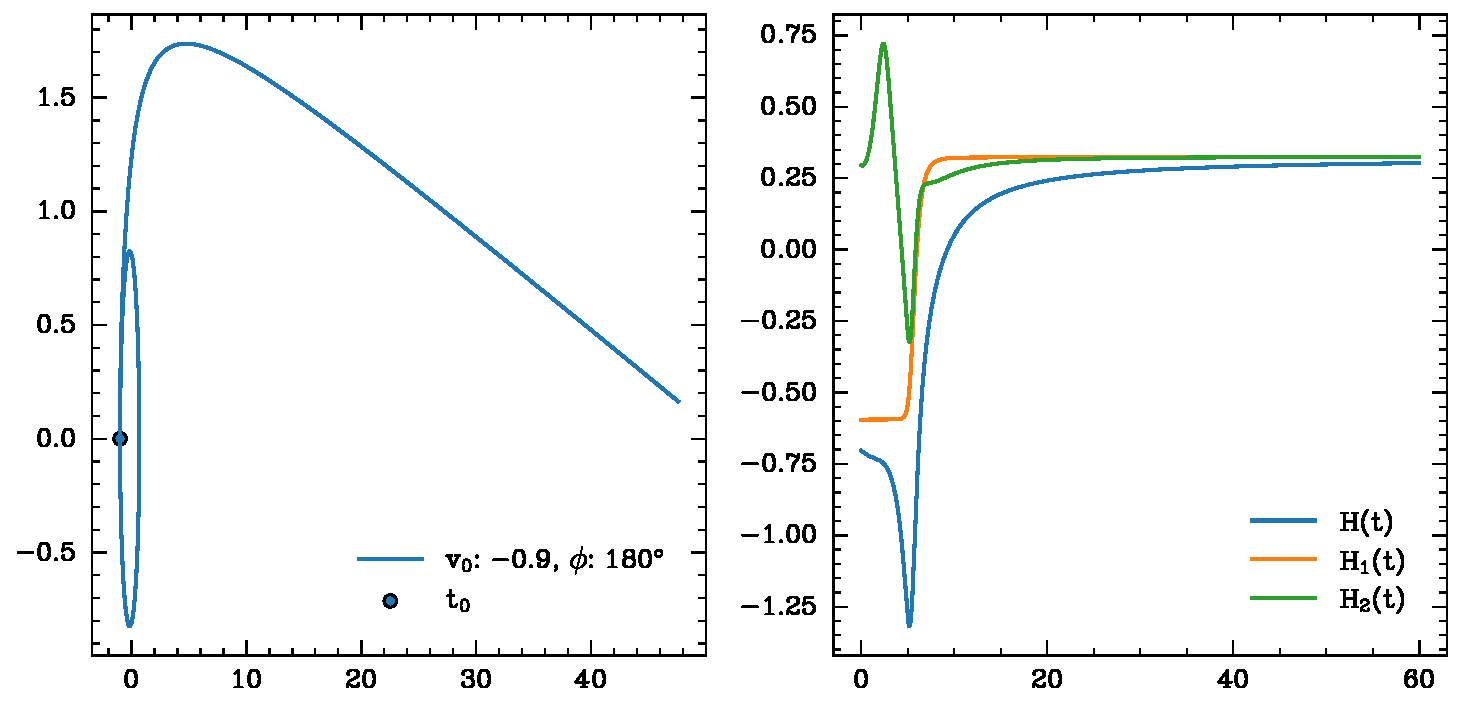
\includegraphics[width=0.9\textwidth]{../images/3-1-60.pdf}
    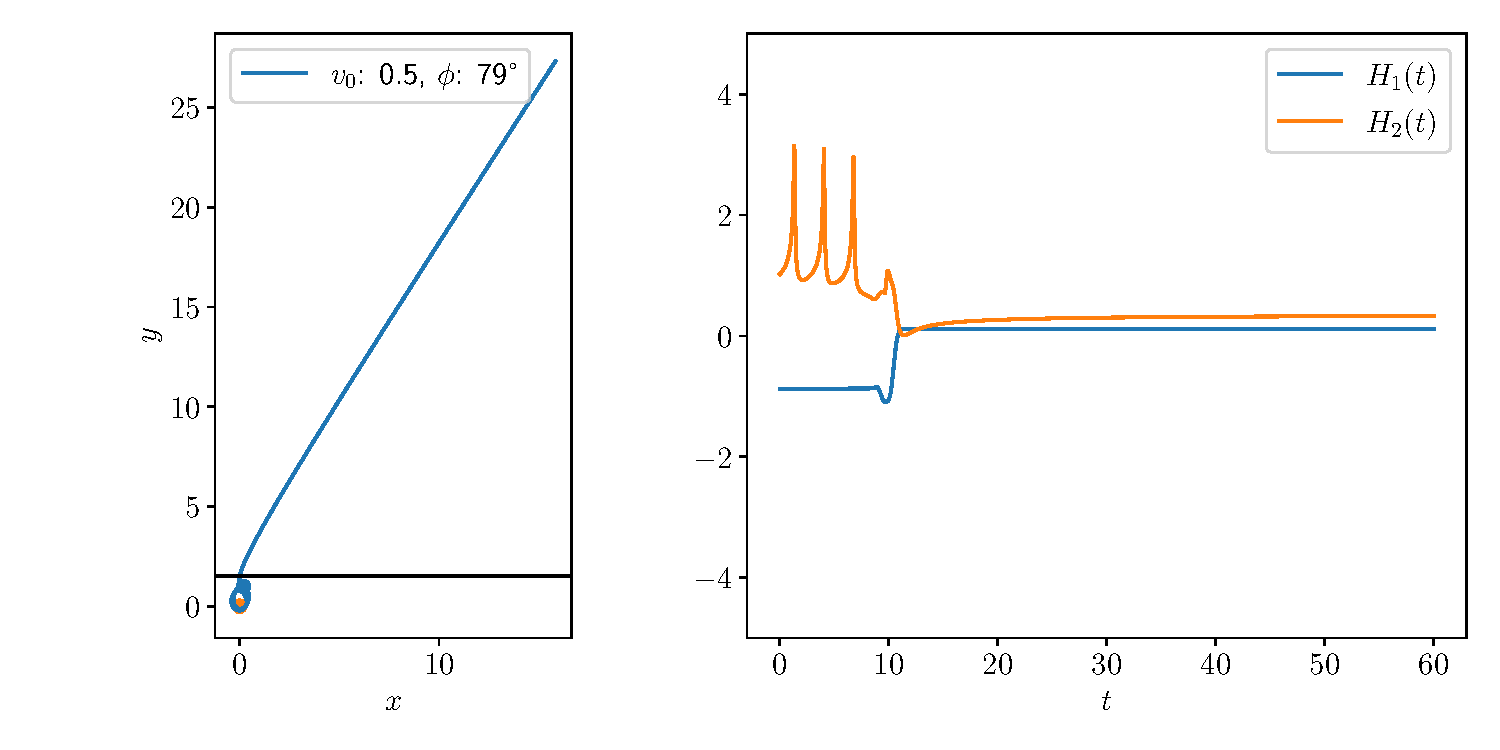
\includegraphics[width=0.9\textwidth]{../images/3-1-7.pdf}\\
    Prelet mimobežne zvezde povzroči razpad prvotnega binarnega sistema.
\end{center}
\begin{center}
    % \includegraphics[width=0.9\textwidth]{../images/3-1-3_.pdf}
    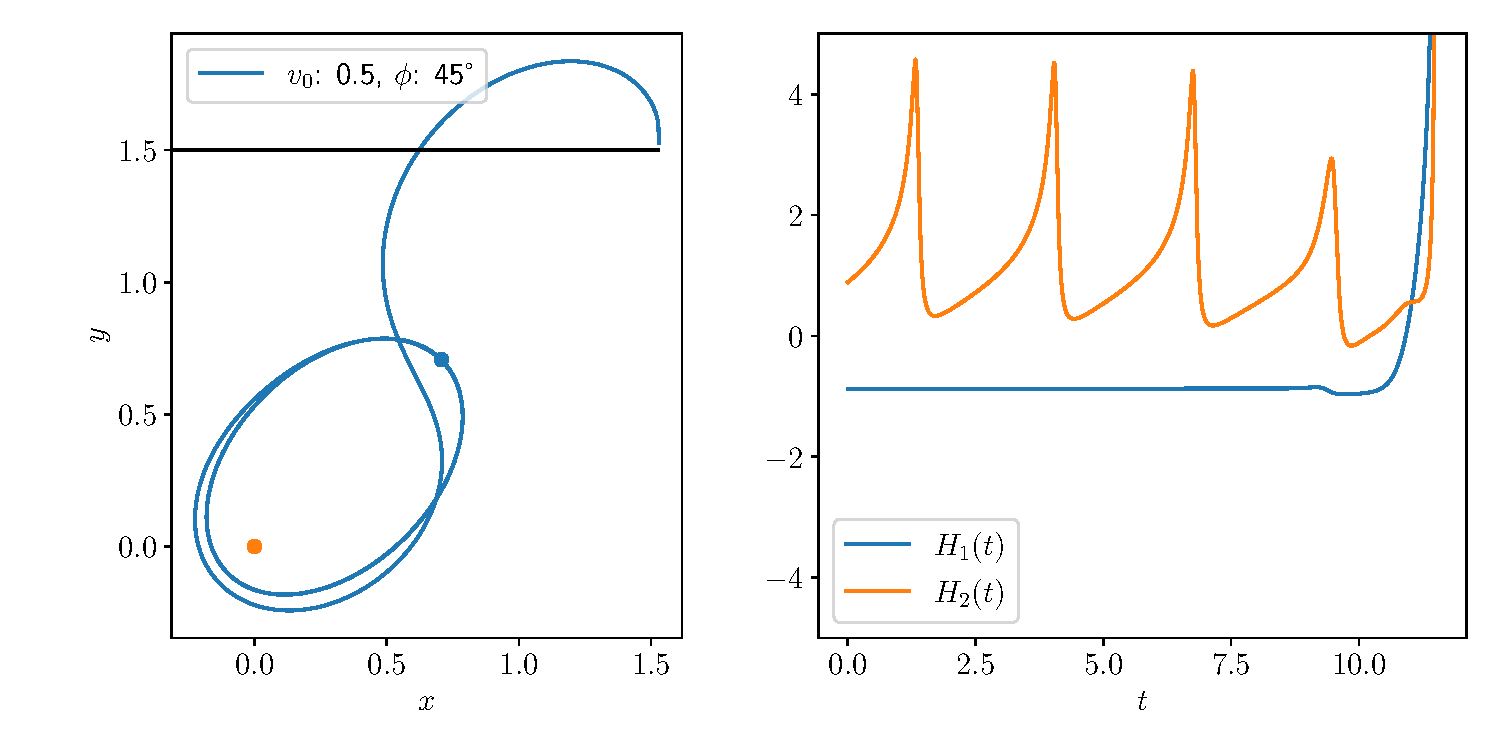
\includegraphics[width=0.9\textwidth]{../images/3-1-4.pdf}\\
    Primer trka planeta v mimobežno zvezdo.
\end{center}
